\section{Schätzen}\label{schaetzen}\script{144}
\textbf{Konsistent} bedeutet, dass wenn Stichprobe vergrössert wird, der Schätzer gegen den wahren Wert strebt. Dabei ist \textbf{Erwartungstreu}, wenn der geschätzte und gemesse Erwartungswert übereinstimmt.

\subsection{Konsistente Schätzer}
Das einfachste Schätzverfahren ist der Mittelwert der Stichprobe.
\[
E(x) = \hat{x} = \frac{1}{N}\cdot \sum\limits_{n=1}^{N}x_n
\]

\subsection{Erwartungstreuer Schätzer}
Für die Varianz gibt der Mittelwert jedoch eine schlechte Schätzung für kleine Stichproben ab. Für grosse Stichproben ist folgender Schätzer erwarungstreu:
\[
\hat{\sigma}^2 = \frac{1}{N-1}\sum\limits_{i=1}^{N}(x_i - \overline{x})^2
\]

\subsection{Maximum Likelihood Prinzip}
Dabei wird eine ML-Funktion $L(\Theta)$ welche anschliessend maximiert wird gebildet. Diese Funktion ist die Partielle Ableitung nach dem gesuchten Schätzparameter der Verteilungsdichte $\hat{\Theta}  = \arg\max\limits_\Theta\{L(x,\Theta)\}$ wobei $L(x,\Theta) := \frac{\partial\Theta}{\partial\varphi}(x)$

\textbf{Beispiel: Normalverteilung}
\[
\hat{\mu} = \frac{1}{n}\sum\limits_{i=1}^{n}x_i \qquad \hat{\sigma}^2  = \frac{1}{N}\sum\limits_{i=1}^{N}(x_i -\mu)^2
\]

\noindent\textbf{Beispiel: Poissionverteilung} \script{150}
\[
\hat{\lambda} = \frac{1}{N}\sum\limits_{i=0}^{N}k_i
\]

\noindent\textbf{Beispiel: Binomialverteilung} \script{150}
\[
\hat{p} = \frac{1}{m\cdot N}\sum\limits_{i=0}^{N}k_i
\]


\subsection{Konfidenzintervall}\script{154}\label{quantilentabelle}
Mit Hilfe eines Schätzers können die Parameter einer Verteilung geschätzt werden. Da der Schätzwert selbst eine Zufallsvariable ist, kann er ziemlich weit weg vom Erwartungswert sein. Das Konfidenzintervall gibt einen Bereich an, wie Wahrscheinlichkeit der Parameter stimmt. 


\begin{center}
	\begin{minipage}{0.20\textwidth}
		\begin{center}
			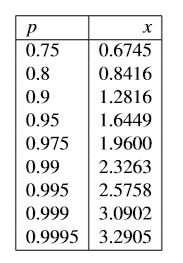
\includegraphics[width=\linewidth,keepaspectratio=true]{Images/quantile-normalverteilung}\\
		\end{center}
	\end{minipage}%%% to prevent a space
	\begin{minipage}{0.3\textwidth}
		\noindent Für \textbf{bekannte} Varianz kann die Quantiellen-Tabelle (links) verwendet werden.\\ ~\\
		\noindent Für \textbf{gschätzte} Varianz wird die t-Tabelle verwendt \script{215}.\\
	\end{minipage}
\end{center}





\noindent\textbf{Beispiel} Siehe Kapitel \ref{konf_intervall}\\

